\documentclass{article}

\usepackage{titlesec}
\titlelabel{\thetitle.\quad}

\usepackage[T1]{fontenc}
\usepackage{inconsolata}

\usepackage[english]{babel}
\usepackage[letterpaper,top=2cm,bottom=2cm,left=2.5cm,right=2.5cm,marginparwidth=1.25cm]{geometry}

\usepackage{hyperref, booktabs, float}
\usepackage[leqno]{amsmath}
\usepackage{enumitem, nccmath,lipsum,amssymb,xcolor,xparse,listings, blindtext}
\usepackage[most]{tcolorbox}

\usepackage{graphicx}
\graphicspath{ {./attachments/} }

\definecolor{light-gray}{gray}{0.9}
\newcommand{\code}[1]{\colorbox{light-gray}{\texttt{#1}}}

\title{Lab 7: Systemd and Package managers}
\author{Mashenkov Timofei B23-CBS-02 \\ \href{mailto:t.mashenkov@innopolis.university}{t.mashenkov@innopolis.university}}
\begin{document}
\maketitle{}

\section{Tracing dependencies}
\noindent

\begin{itemize}
	\item \code{graphical.target}
	      \begin{itemize}
		      \item 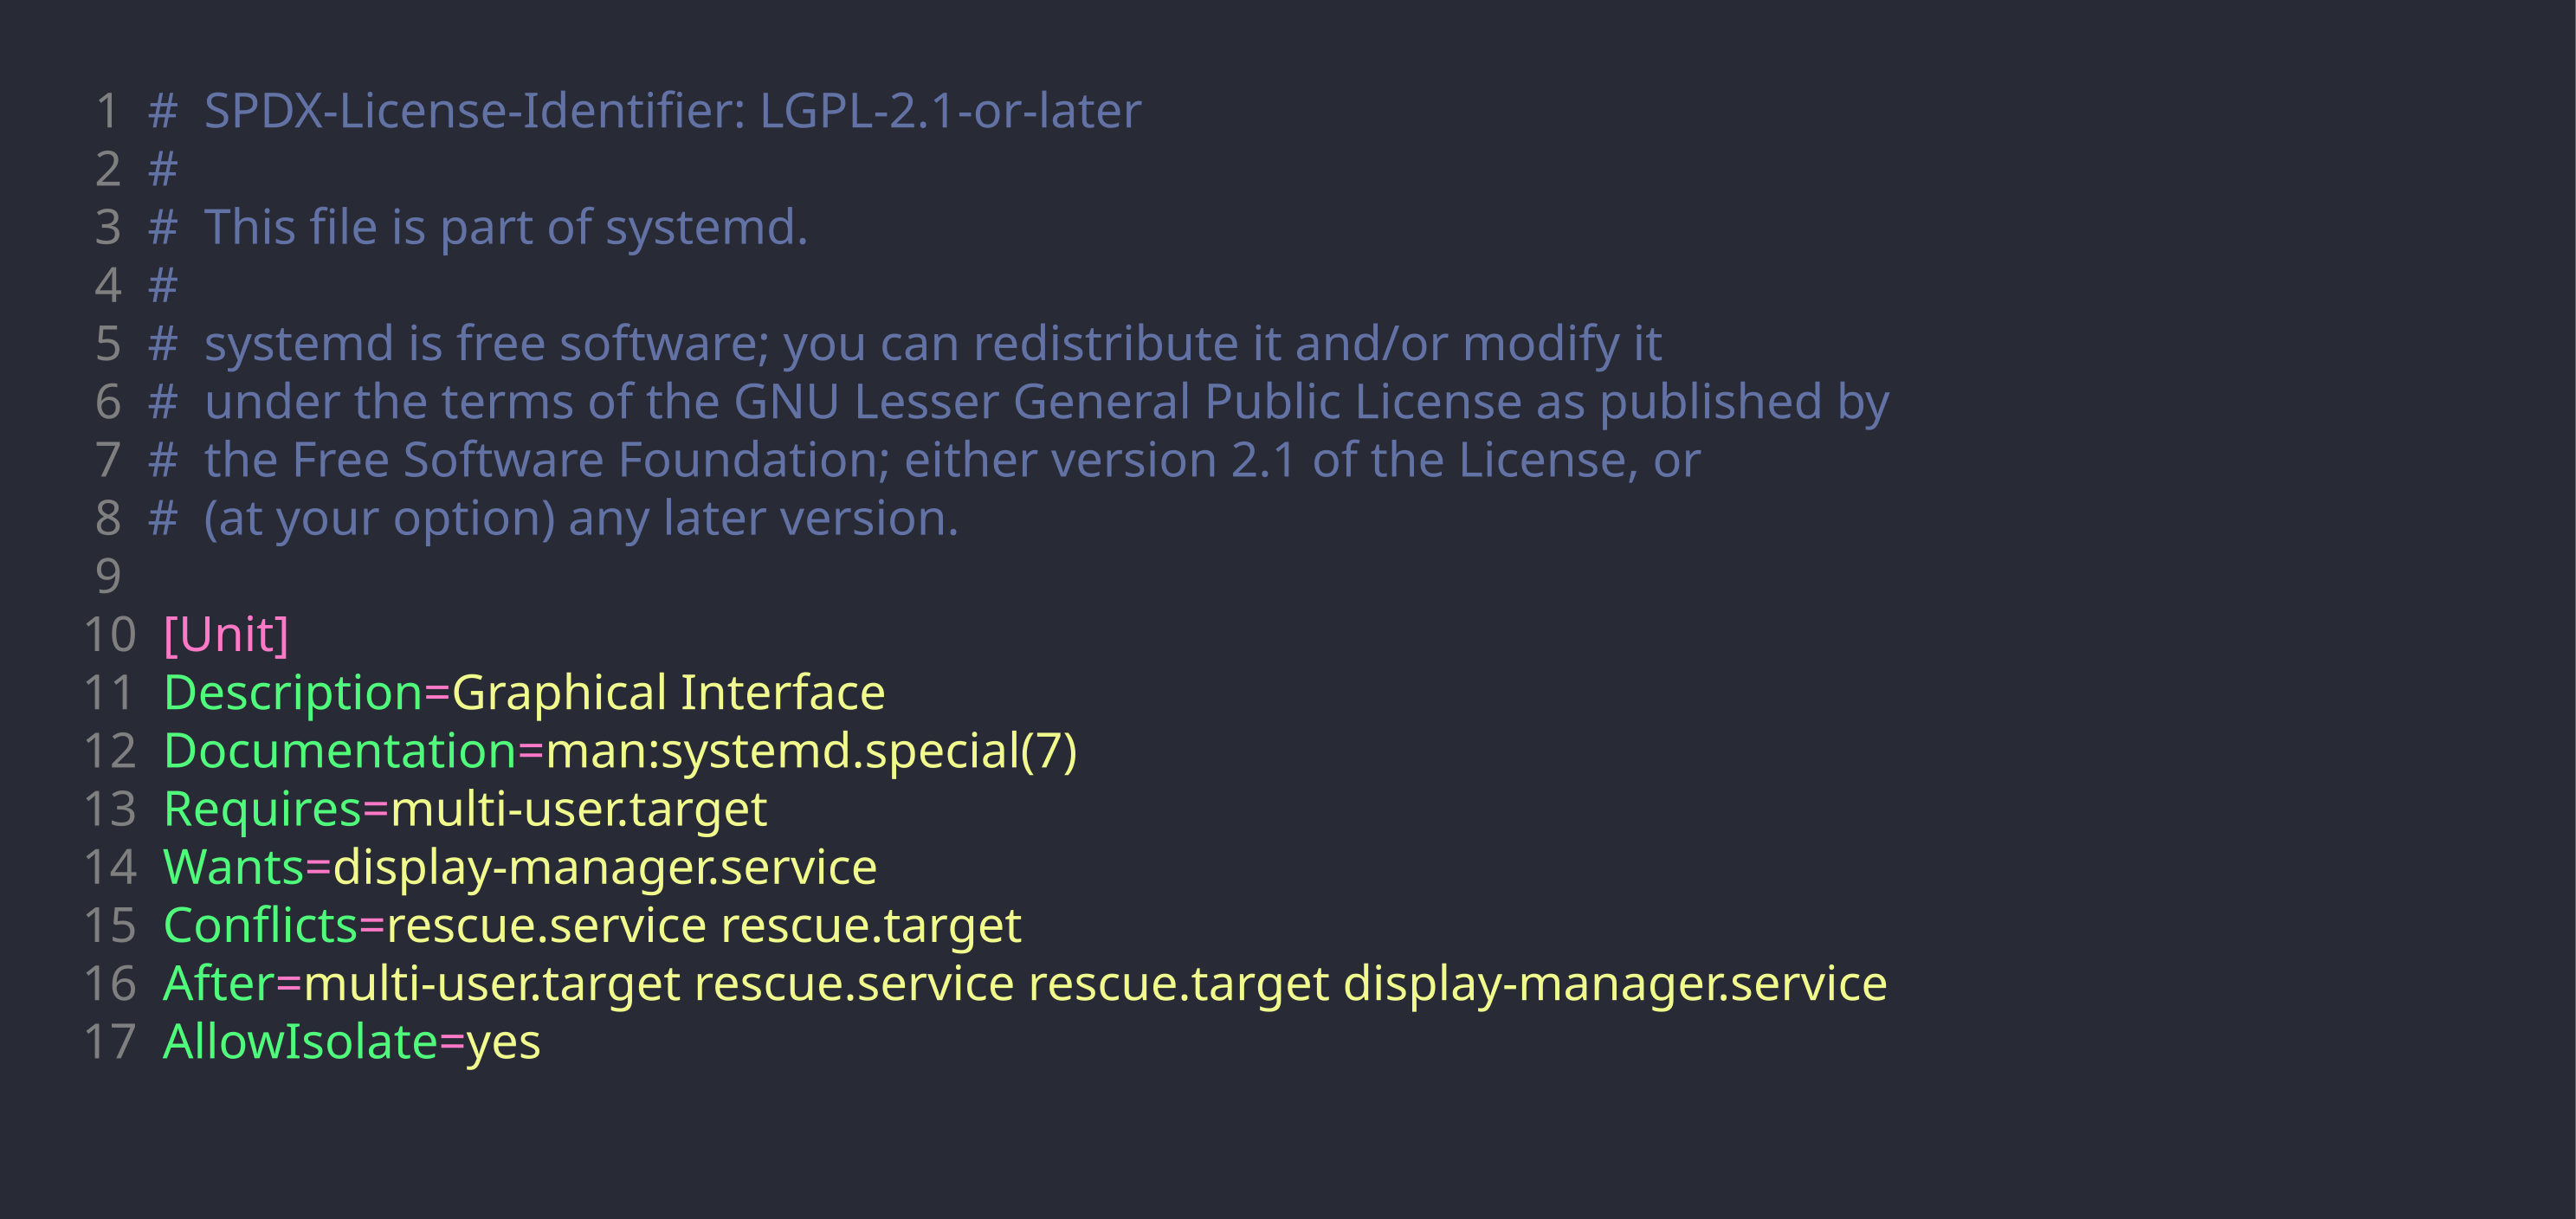
\includegraphics[width=240pt]{7_1.jpg}
		      \item \textbf{Purpose:} Starts the GUI environment.
	      \end{itemize}
	\item \code{multi-user.target}
	      \begin{itemize}
		      \item 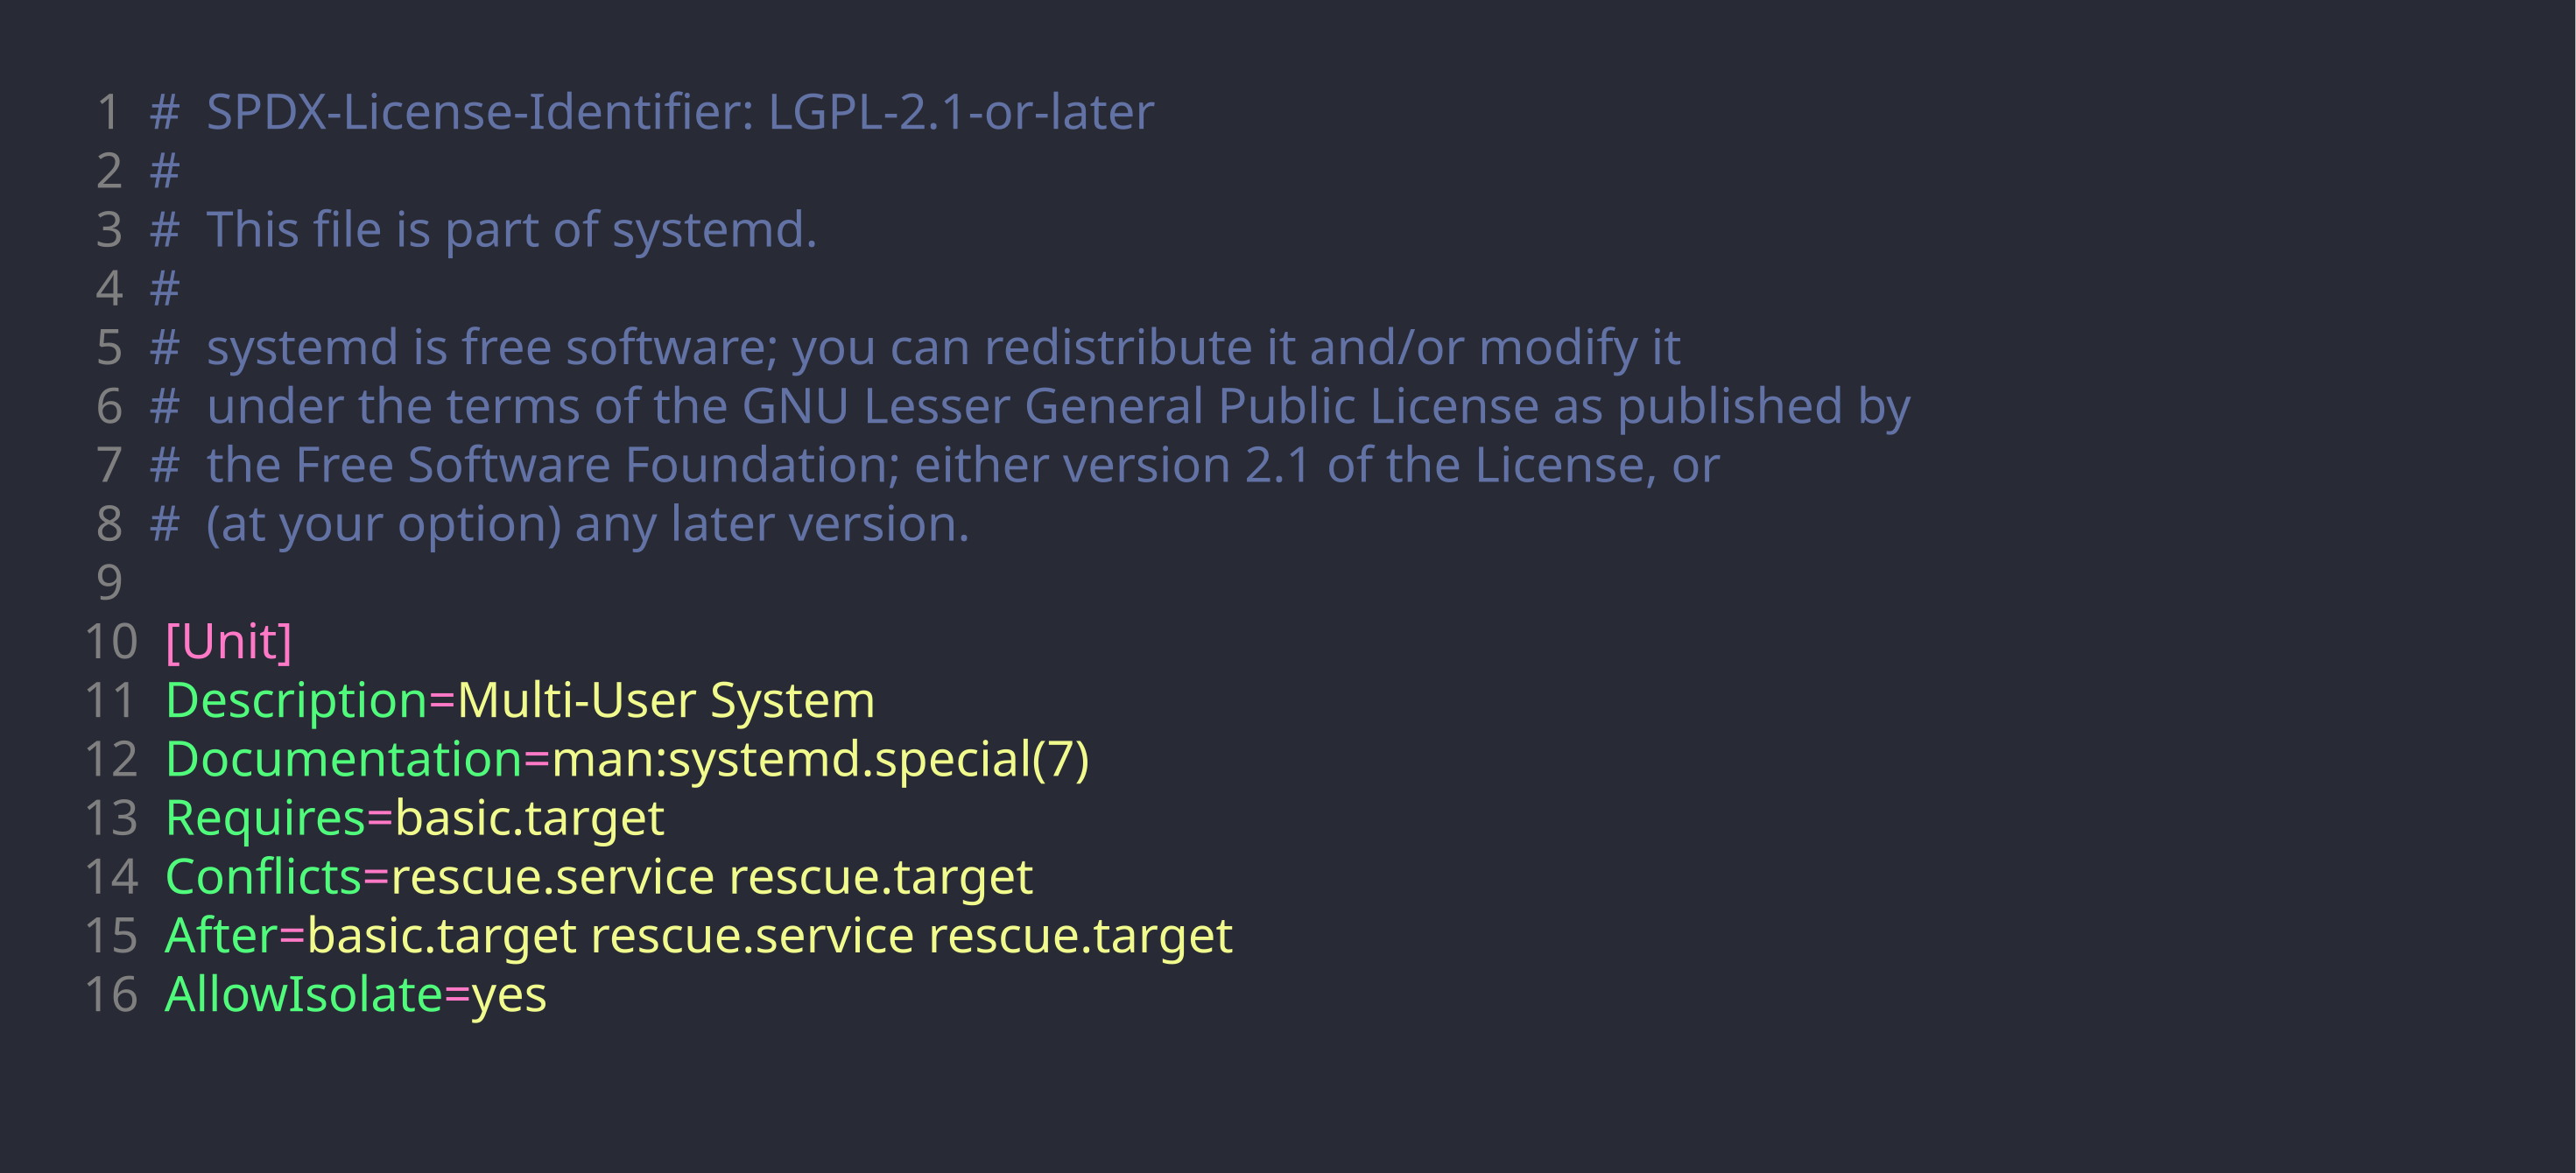
\includegraphics[width=240pt]{7_2.png}
		      \item \textbf{Purpose:} Non-graphical multi-user system.
	      \end{itemize}
	\item \code{basic.target}
	      \begin{itemize}
		      \item 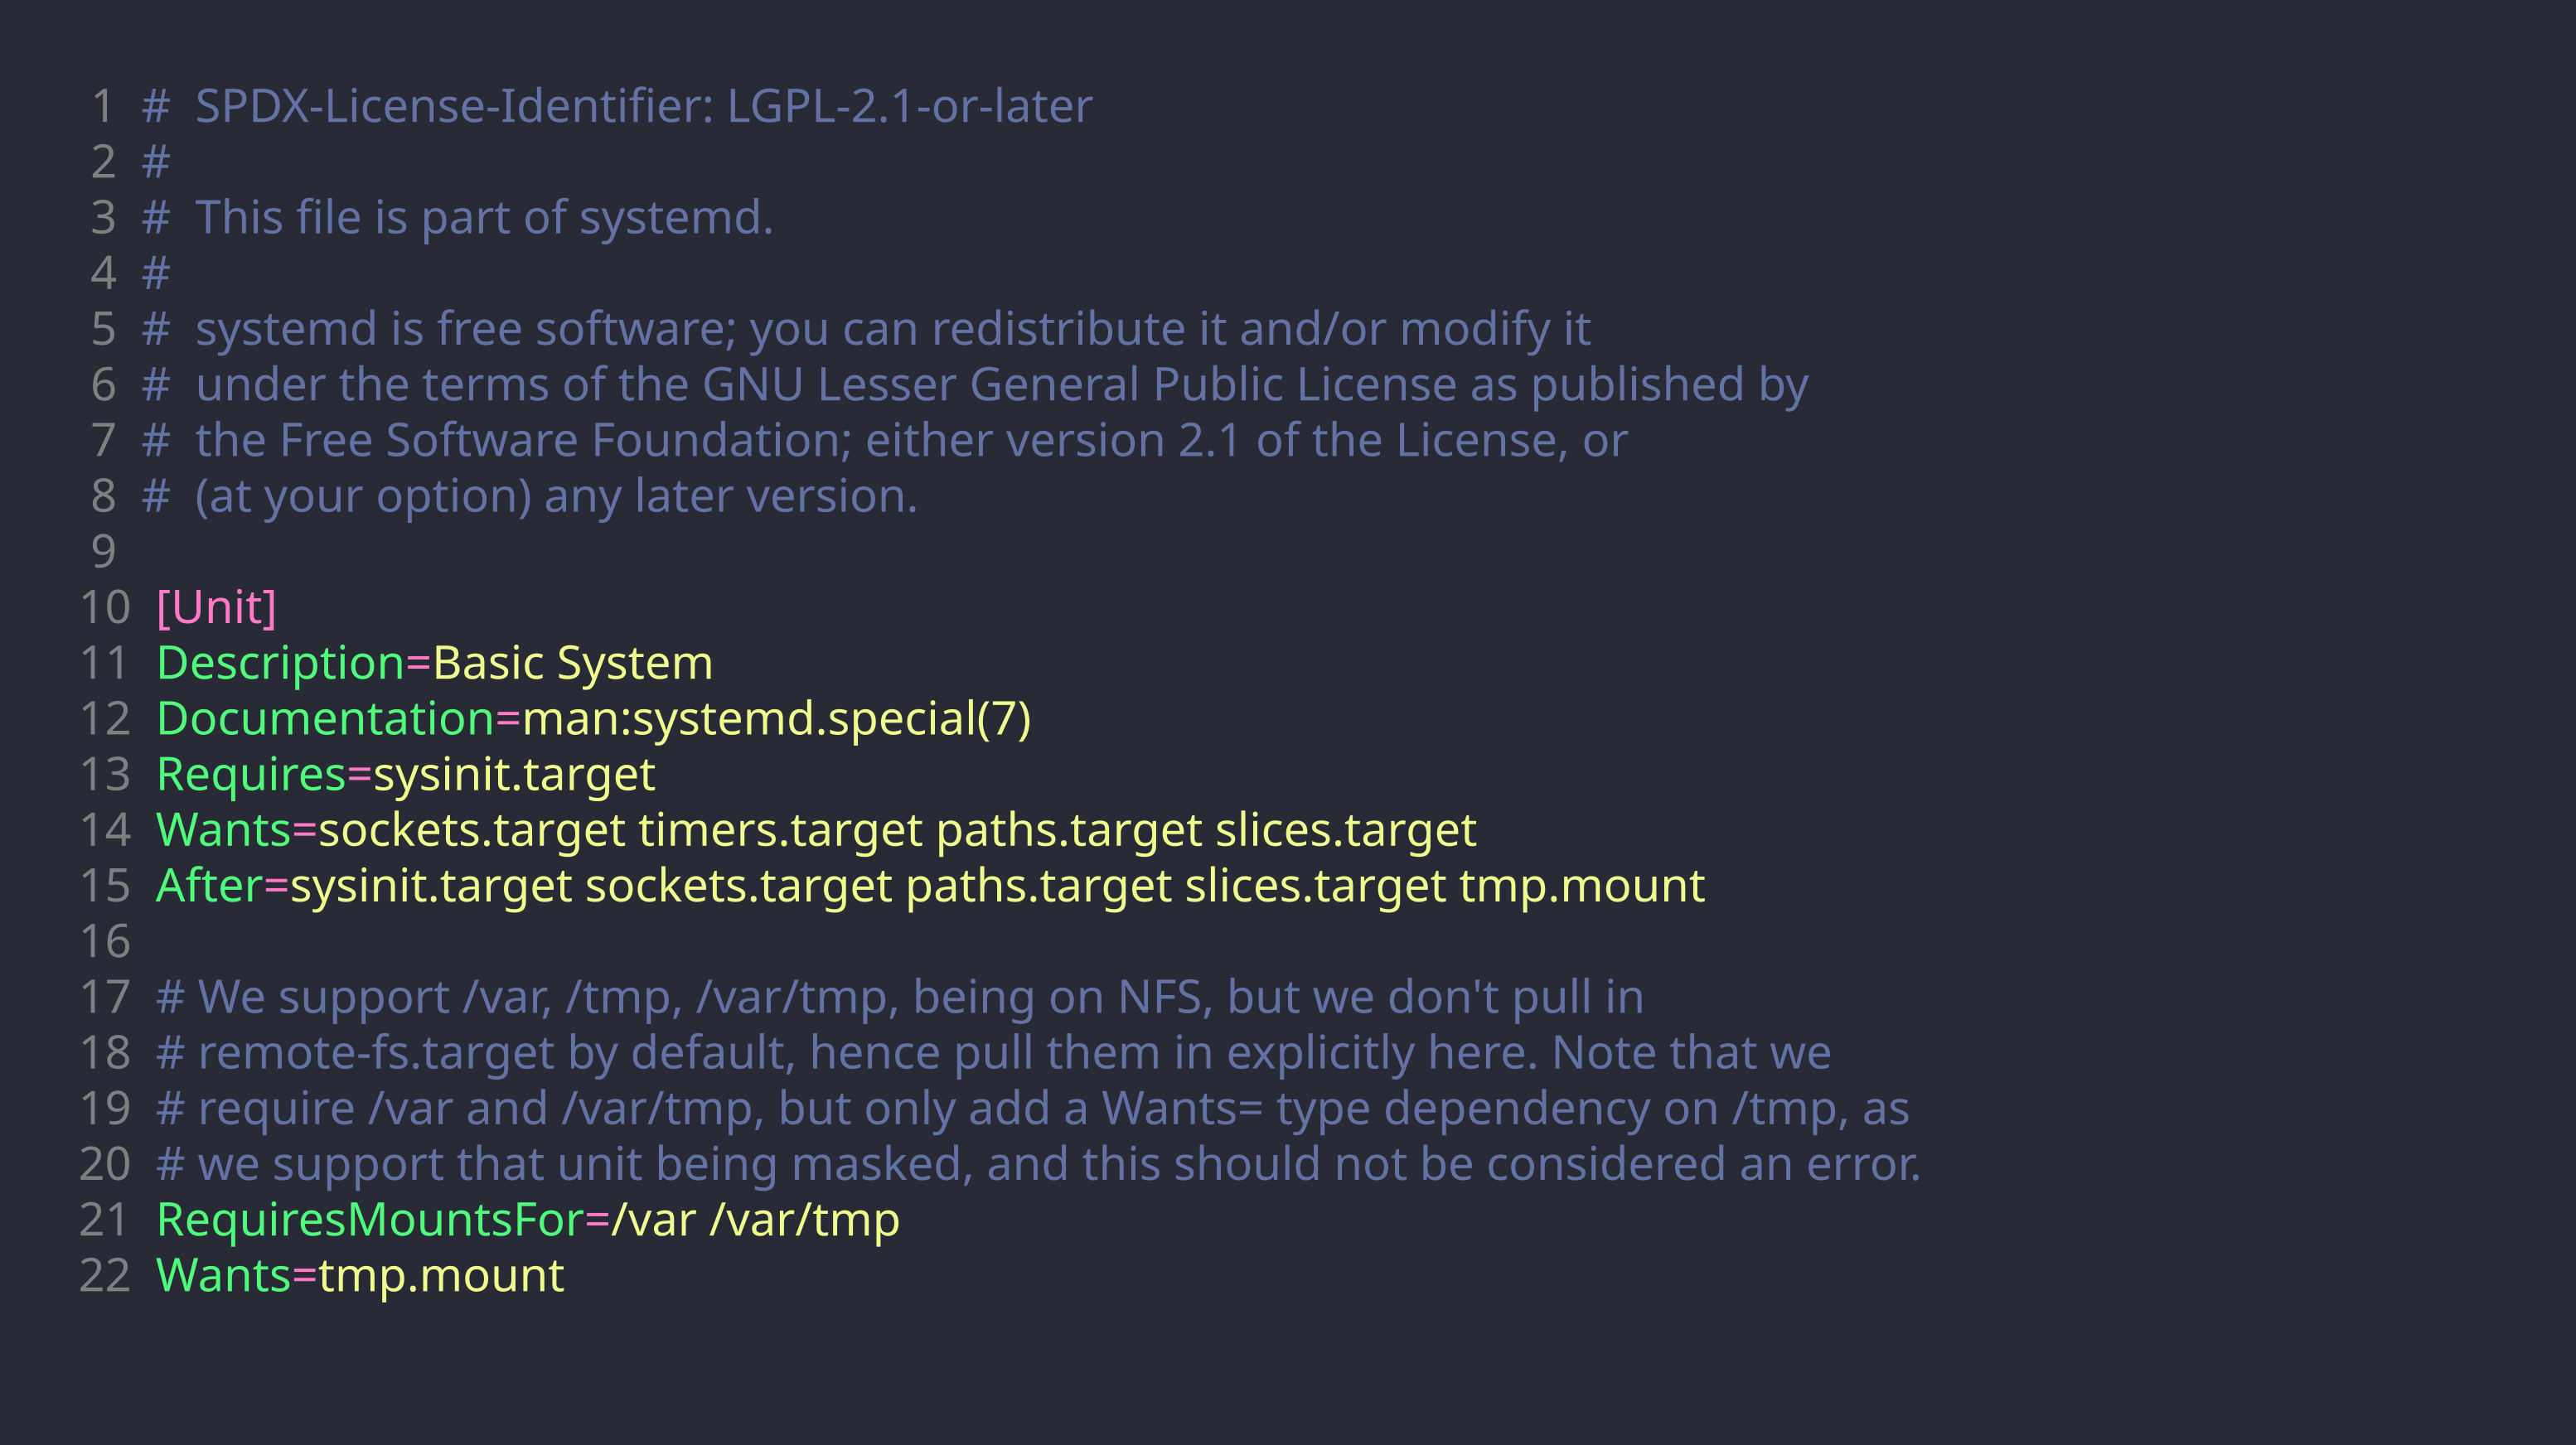
\includegraphics[width=240pt]{7_3.png}
		      \item \textbf{Purpose:} Basic system initialization.
	      \end{itemize}
	\item \code{sysint.target}
	      \begin{itemize}
		      \item 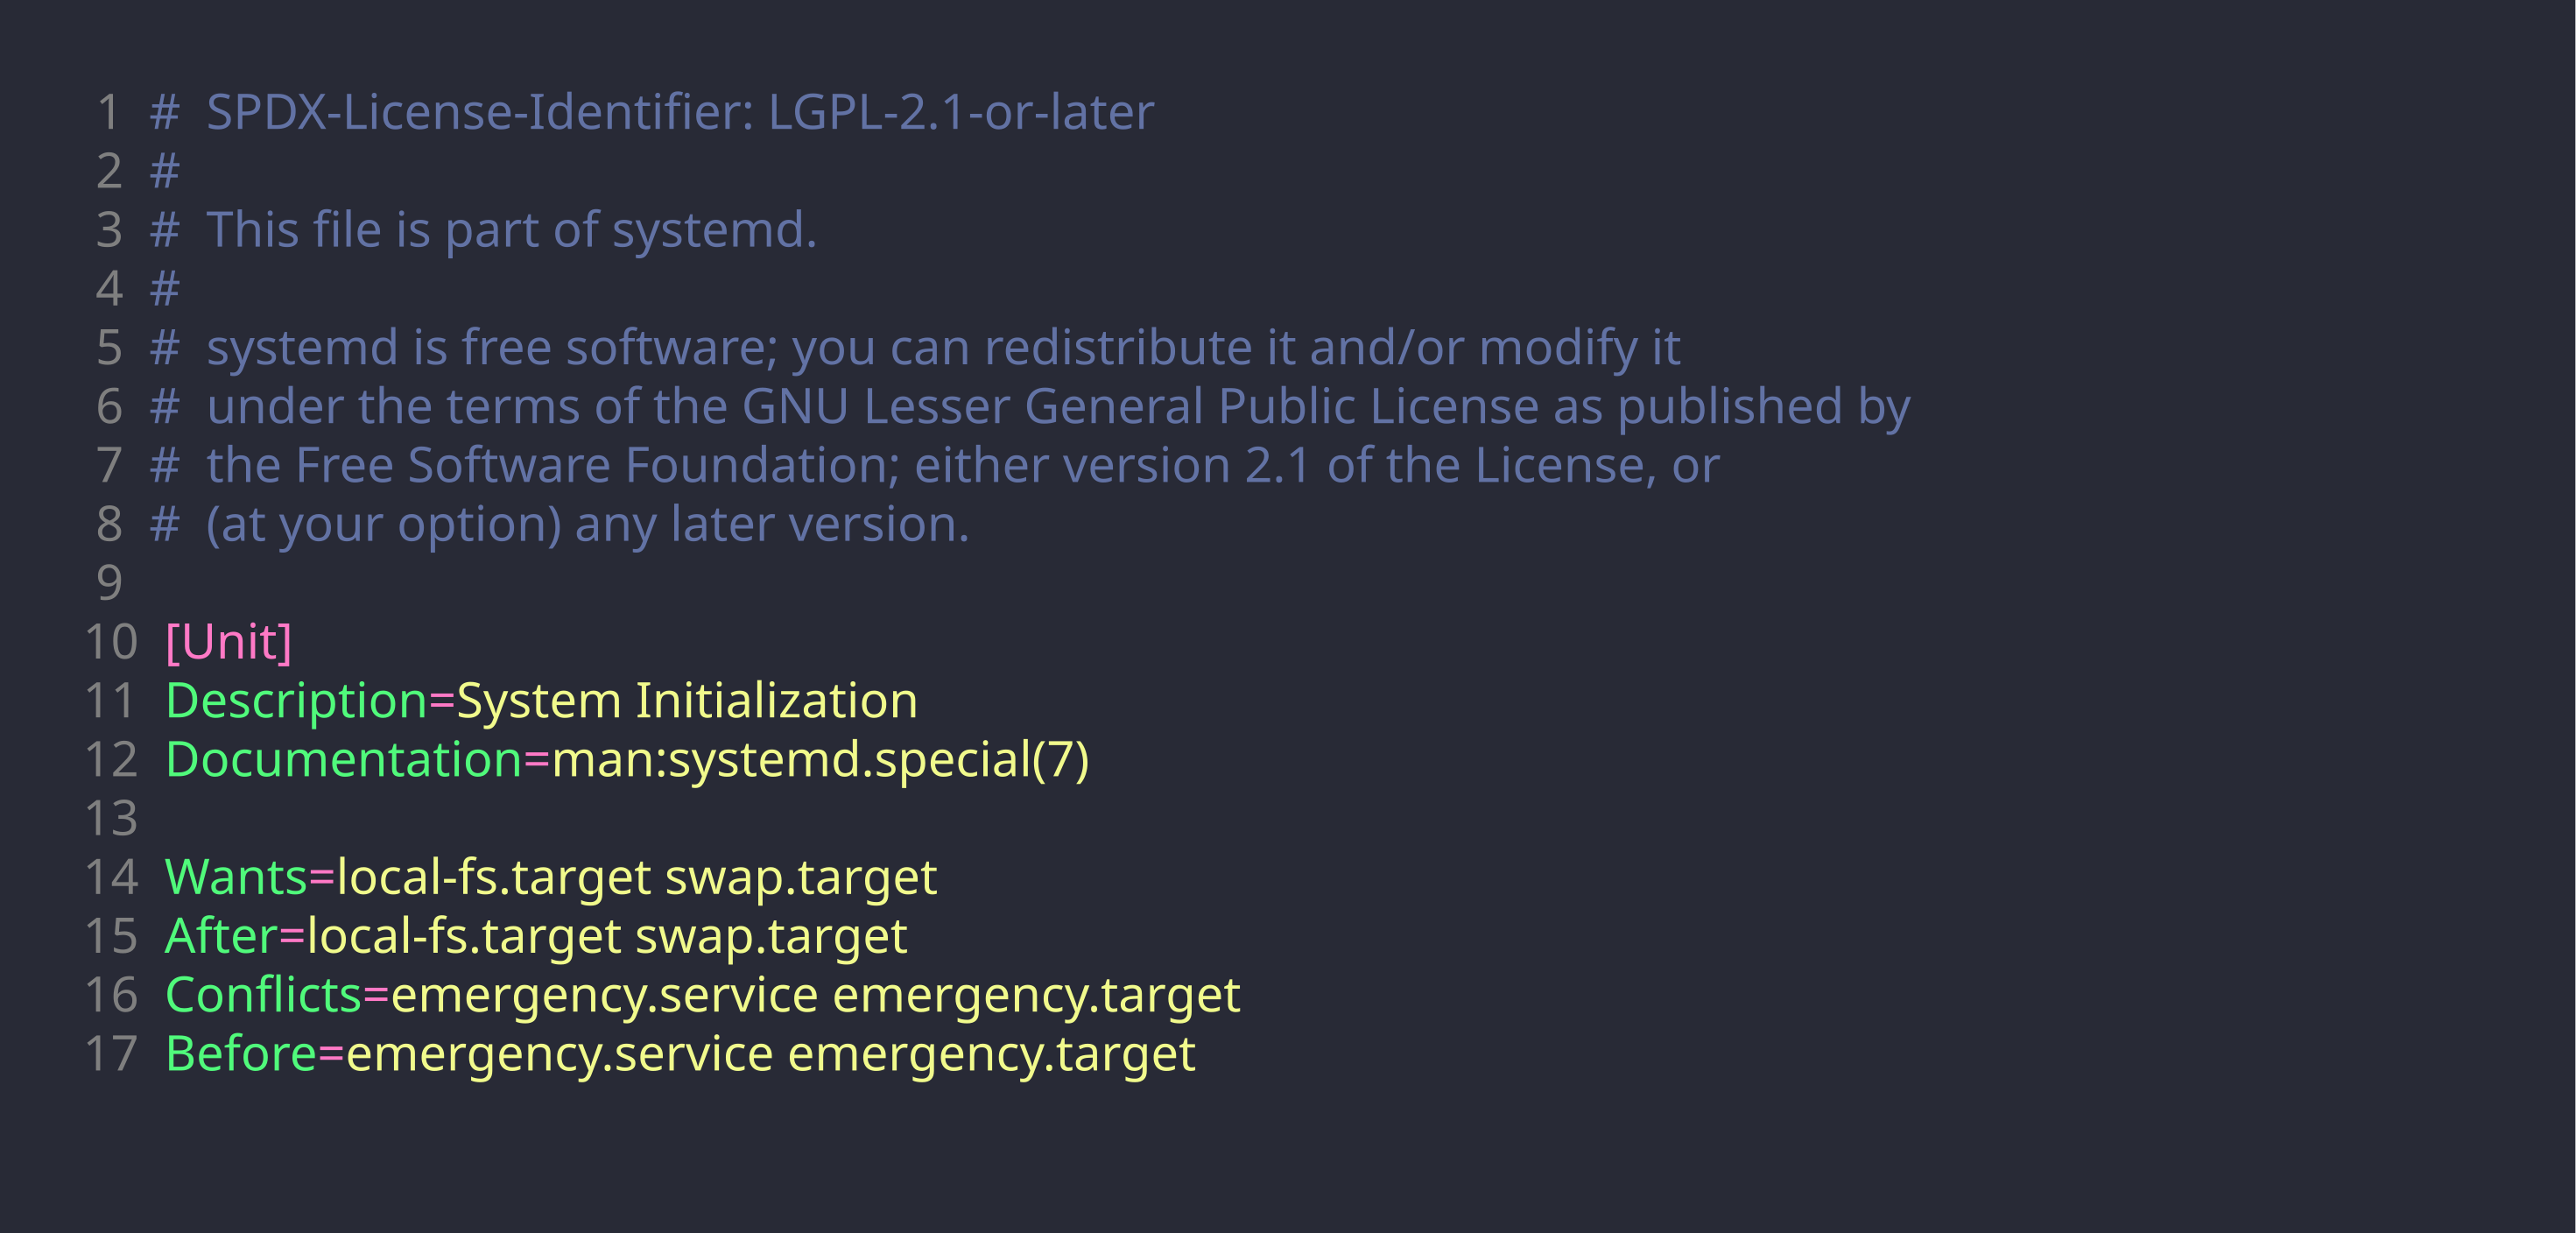
\includegraphics[width=240pt]{7_4.png}
		      \item \textbf{Dead end}
		      \item \textbf{Purpose:} Mounts filesystems and swaps.
		      \item \textbf{Wants:} Mount units
		      \item \textbf{Why whants?} To attempt mounting filesystems but continue if they fail.
	      \end{itemize}
\end{itemize}

\section{Bash Web Server}
\noindent

\begin{figure}[H]
	\centering
	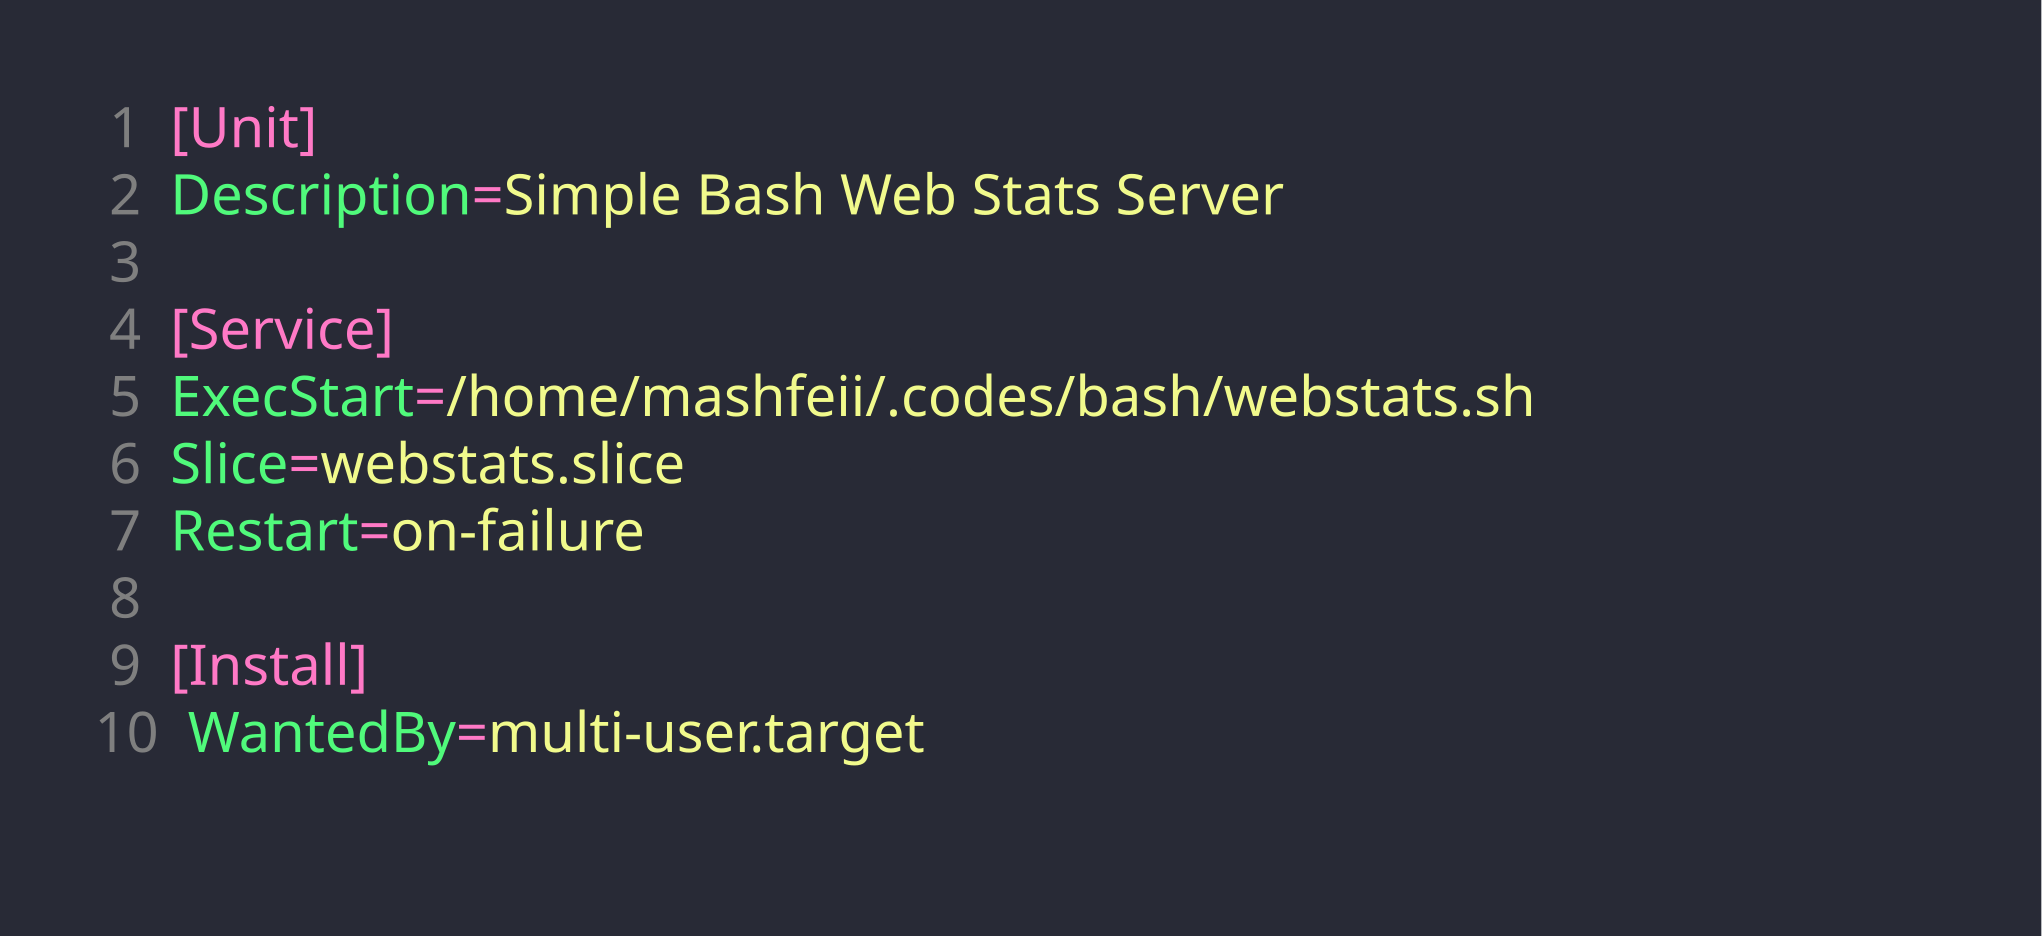
\includegraphics[width=240pt]{7_5-1.png}
	\caption{\code{/lib/systemd/system/webstats.service}}
\end{figure}

\begin{figure}[H]
	\centering
	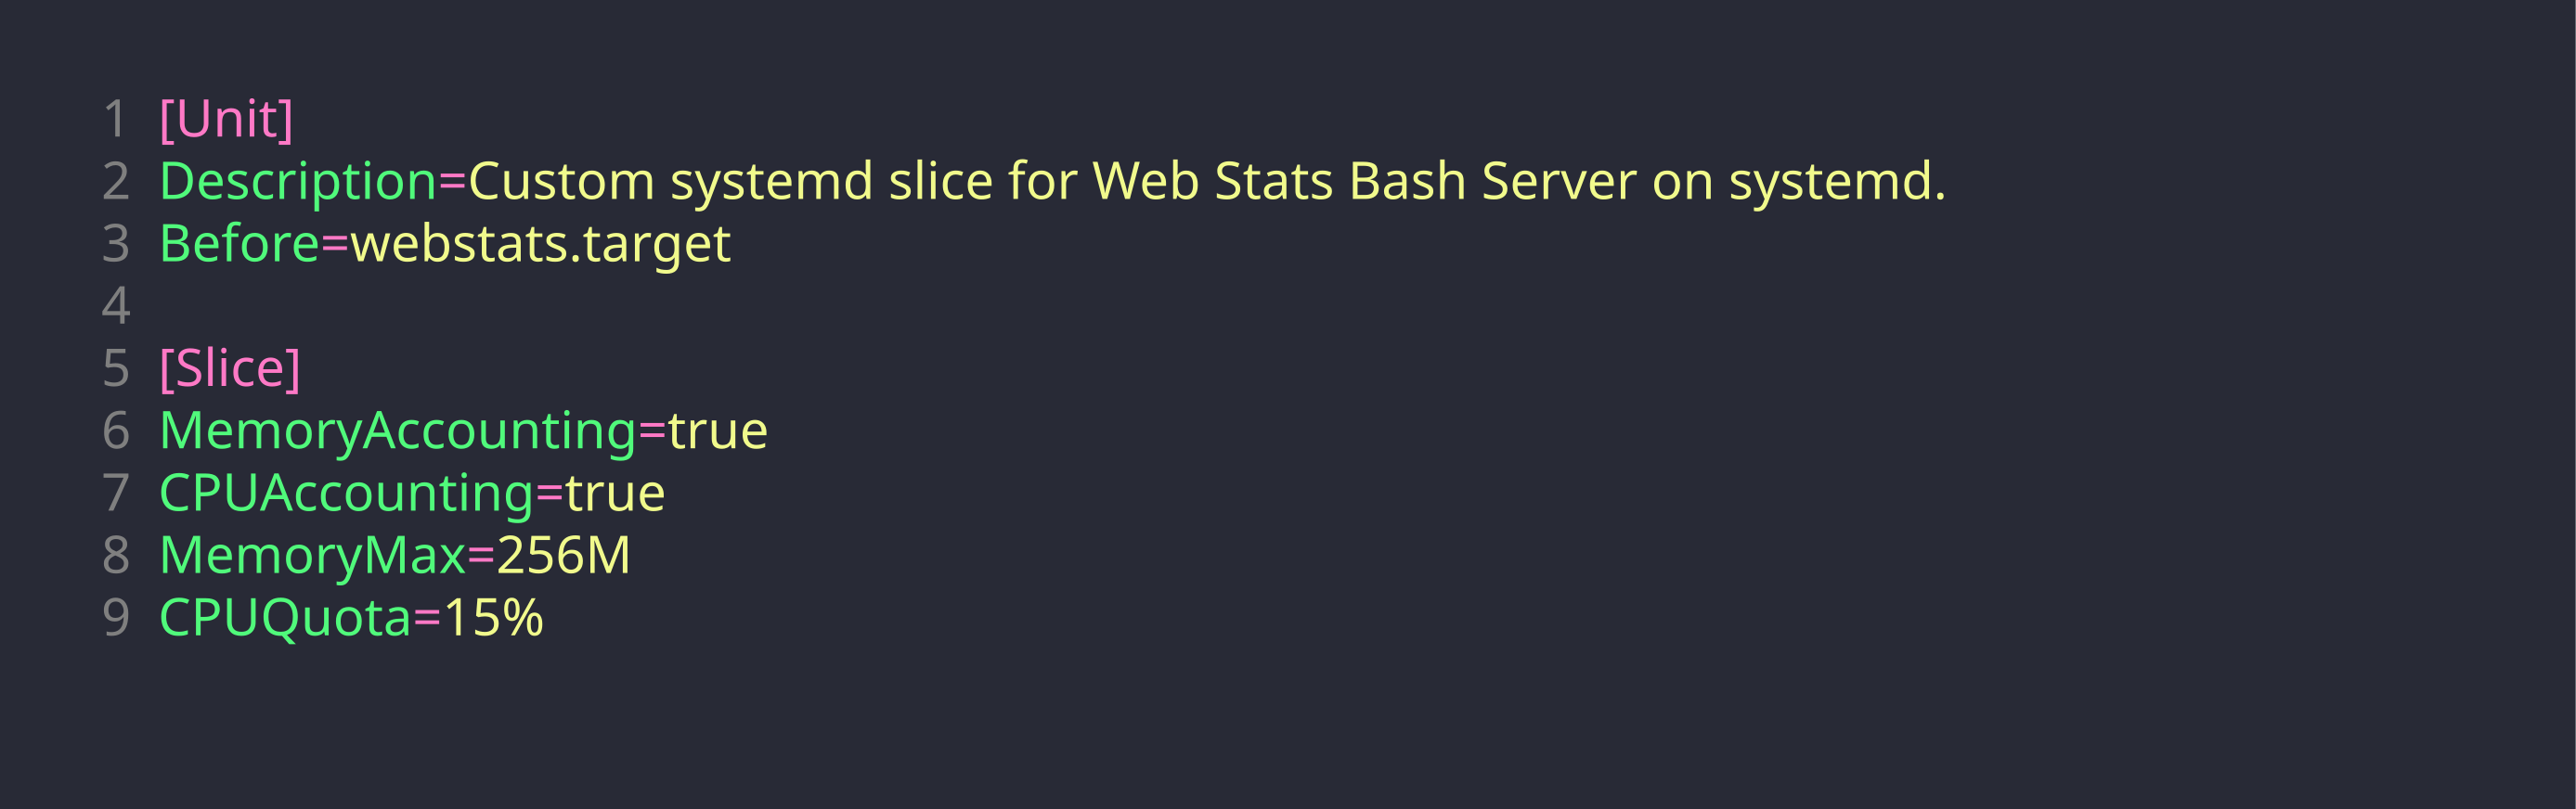
\includegraphics[width=240pt]{7_5-2.png}
	\caption{\code{/lib/systemd/system/webstats.slice}}
\end{figure}

\begin{figure}[H]
	\centering
	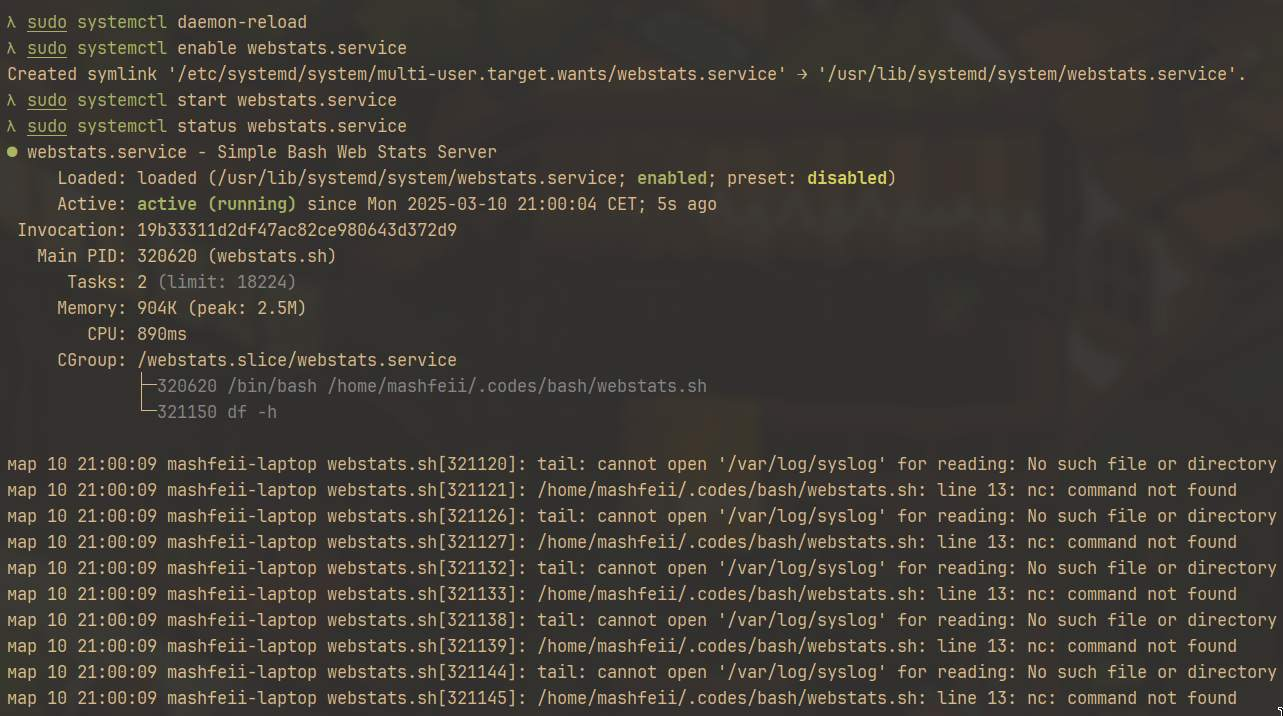
\includegraphics[width=460pt]{7_5-3.jpg}
	\caption{Enabling and starting the service\label{fig:7_5-3}}
\end{figure}

Since my working distribution is Arch-based, file \code{var/log/syslog} is not presented by default \ref{fig:7_5-3}, but the script remains to follow initial requirements.

\newpage
\section{Upgrade VS Full-Upgrade}
\noindent

\begin{itemize}
	\item \code{apt updgrade} - upgrade all packages that can be upgraded without installing additional packages or removing conflicting installed packages.
	\item \code{apt full-upgrade} - upgrade the packages, the kernel, and remove conflicting packages or install new ones.
\end{itemize}

\code{apt full-upgrade} can remove used dependencies, which can significantly complicate or even break the usual workflow.

\section{Ubuntu Package}
\noindent

\begin{figure}[H]
  \centering
  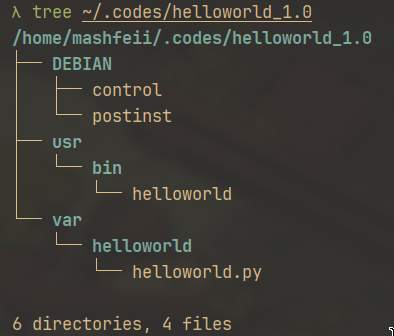
\includegraphics[width=240pt]{8_2.jpg}
  \caption{Tree structure of the package}
\end{figure}

\begin{figure}[H]
  \centering
  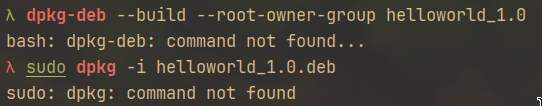
\includegraphics[width=240pt]{8_1.jpg}
  \caption{Building steps of the package}
\end{figure}

The structure of the package is quite simple, but to fullfill the task I probably should build the package for Arch using \code{PKGBUILD} and \code{makepkg} :).

\section{Bonus: Custom Target}
\noindent

\begin{figure}[H]
  \centering
  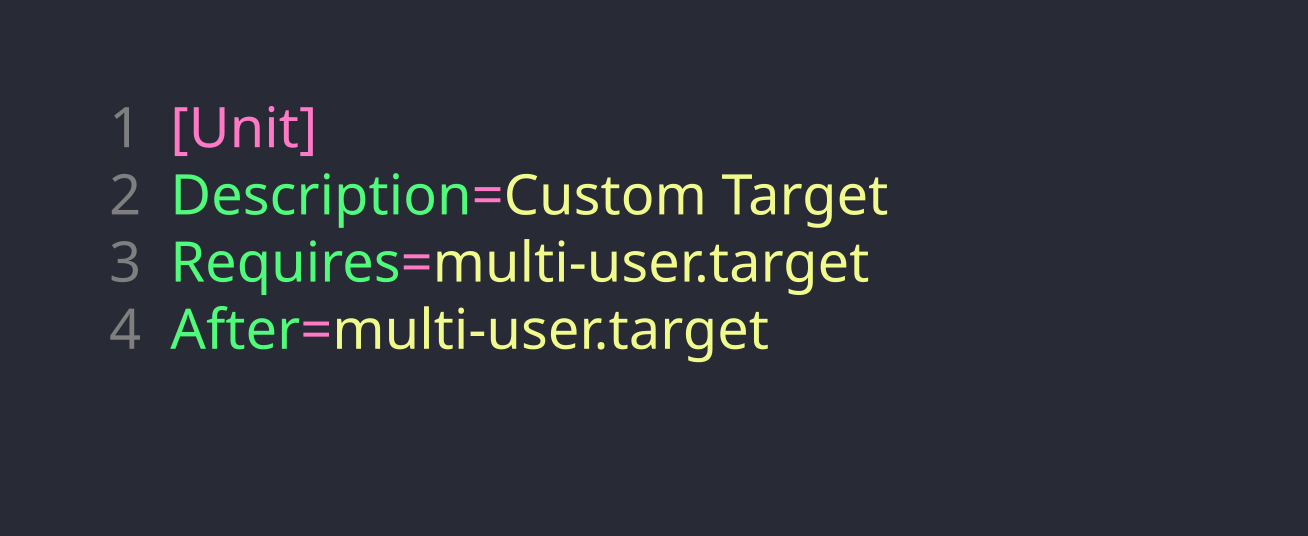
\includegraphics[width=240pt]{9_1.png}
  \caption{\code{/lib/systemd/system/custom.target}}
\end{figure}

\begin{figure}[H]
  \centering
  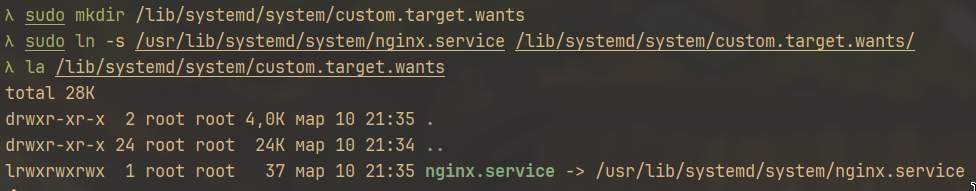
\includegraphics[width=460pt]{9_2.jpg}
  \caption{Creating symlink to the custom target's wants}
\end{figure}

\section{Bonus: RPM Package}

\begin{figure}[H]
  \centering
  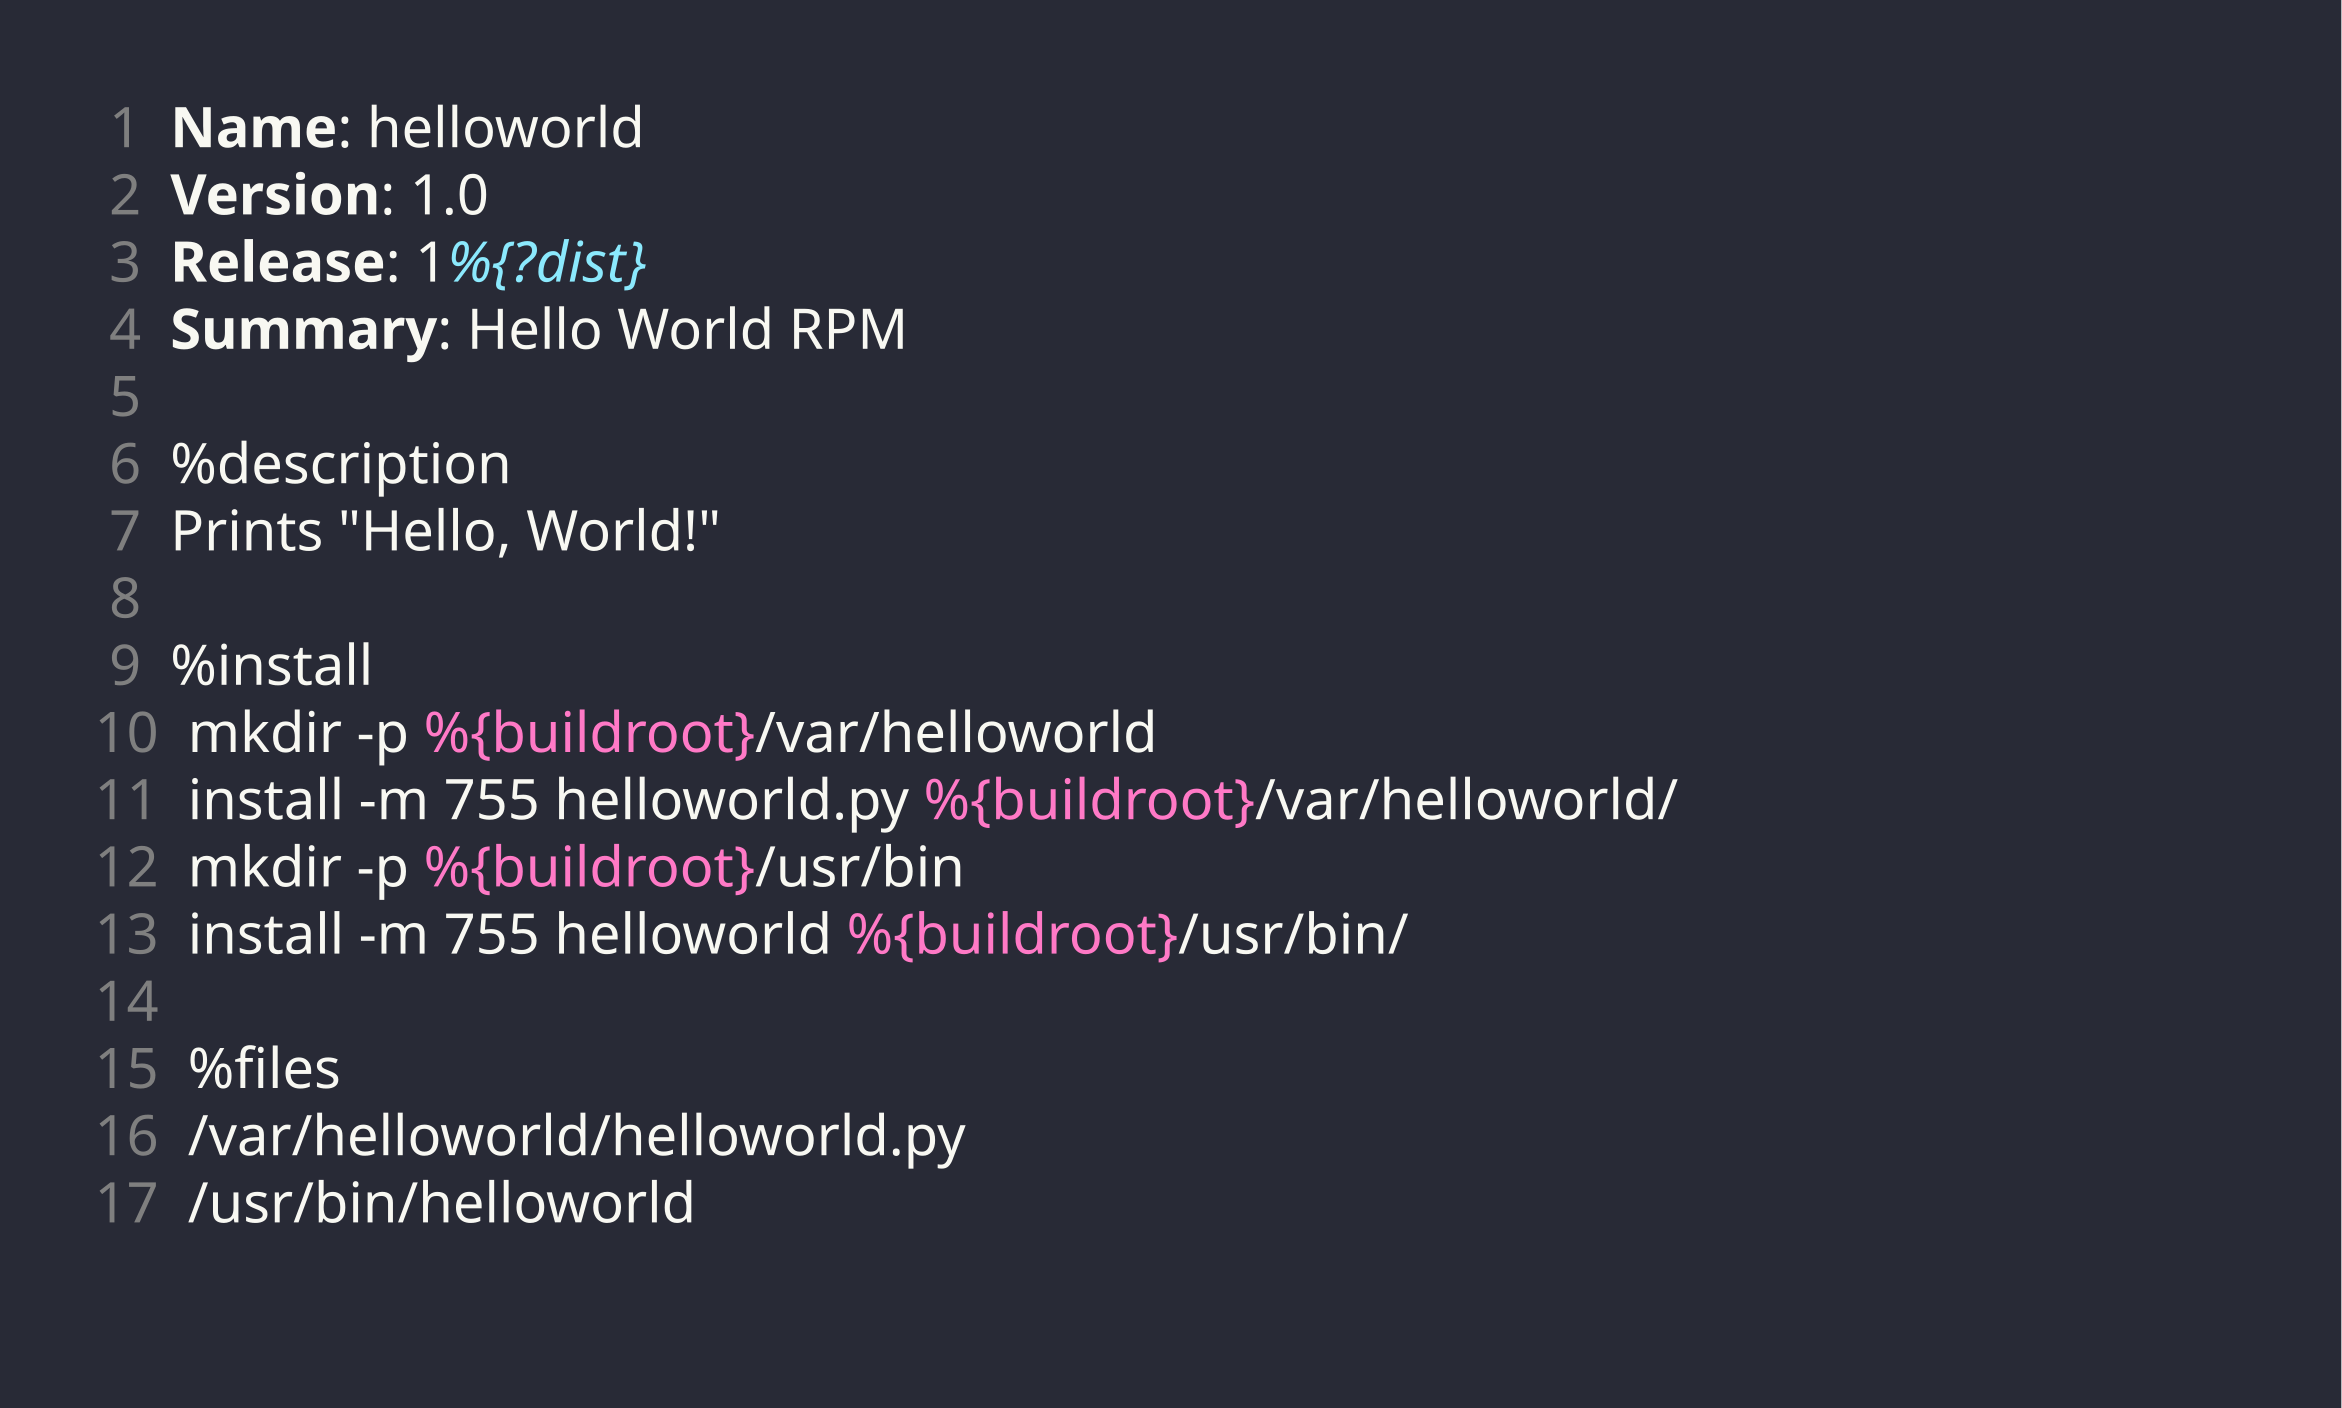
\includegraphics[width=320pt]{10_1.png}
  \caption{\code{helloworld.spec}}
\end{figure}

Building the package: \code{rpmbuild -bb helloworld.spec}

\end{document}
